\section{Memory Bus Speed Sensitivity}
\label{sec:results:bus_sensitivity}


\begin{figure}[t]
    \centering
    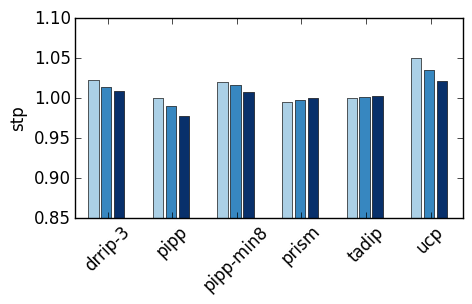
\includegraphics[scale=0.7]{figures/results/speedup/membus-stp-06_4-all-membus}
    \caption[Speedup with decreasing bus bandwidth]{Speedup of cache partition algorithms normalized to LRU with decreasing memory bus bandwidth}
    \label{fig:results:bus}
\end{figure}

In this experiment, we explore how changes to the memory bus bandwidth affect the performance of the cache partitioning algorithms.
With lower bandwidth, we expect that memory requests will take longer to complete, also we expect memory queue times to increase in periods with high utilization.
However, we know that increased memory latency does not necessarily imply lower performance, as the OOO-core may be able to hide the increased memory latency.
We also know that increasing the memory latency may have an impact on the amount of speculative execution performed by the cores.
As a result, we might see a change in the number of memory requests and also MPKI in our experiments.
For this experiment, we use the same base system as in all previous experiments, and we utilize all our 4-core workloads.
The memory bus bandwidth is varied, from the standard 6.4GB/s down to 3.2GB/s and 1.6GB/s.

Figure~\ref{fig:results:bus} show average STP of all 4-core workloads for each algorithm.
TADIP shows no sensitivity to reduced memory bandwidth, both the STP measurements shown in the figure and the MPKI measurements are about equal in all cases.
The results for DRRIP show a slightly better performance compared to LRU with reduced memory bandwidth.
UCP has the best speedups in this experiment, increasing from about 4.8\% in the base case to about 7\% with reduced memory bandwidth.
The only algorithm that shows a decline in performance measured in STP is PriSM.
However, the HMS measurements for PriSM show a steady increase from about 2\% better than LRU in the base case to about 4\% in the most constrained case.
This indicates that some of the benchmarks are seeing a performance improvement, while others are slowed down enough to affect the STP measurements negatively.
For the two final algorithms, PIPP, and PIPP-min8, we see a slight performance improvement.
Most notably we see that PIPP performs as good as LRU in the most constrained case.
The performance development in PIPP-min8 mimics that of PIPP, which has been shown to be the case in several previous experiments.
PIPP-min8 outperforms both PIPP and LRU.

\begin{figure}[t]
    \centering
        \begin{subfigure}[b]{0.5\textwidth}
            \includegraphics[scale=0.8]{figures/results/speedup/membus-0_5M-stp-06_4-ucp-membus}
            \caption{STP.}
            \label{fig:results:bus-05:ucp:stp}
        \end{subfigure}%
        \begin{subfigure}[b]{0.5\textwidth}
            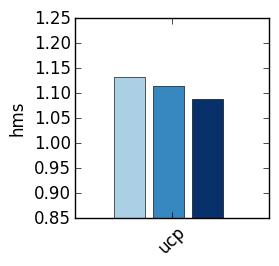
\includegraphics[scale=0.8]{figures/results/speedup/membus-0_5M-hms-06_4-ucp-membus}
            \caption{HMS.}
            \label{fig:results:bus-05:ucp:hms}
        \end{subfigure}
        \caption{Speedup of UCP normalized to LRU with reduced L3 cache.}
        \label{fig:results:bus-05:ucp}
\end{figure}


In all our experiments, we have shown that UCP outperforms the other implemented algorithms.
Both when reducing the available memory bandwidth in this experiment, and when we reduced the size of the LLC in Section~\ref{sec:results:l3size_sensitivity}, UCP has show improved performance over LRU.
Because of this, we ran an additional experiment varying the memory bandwidth, but this time utilizing the lowest cache configuration used in Section~\ref{sec:results:l3size_sensitivity}, 0.5MB.
Because of the time constraints on this thesis, we only have results for UCP compared to LRU.
Figure~\ref{fig:results:bus-05:ucp} shows the speedup for UCP compared to LRU with varying memory bus bandwidth.
These results show that when we combine the high cache pressure caused by reduced LLC size, with increased memory latency, UCP can outperform LRU greatly.
Our results show UCP performing more than 21\% better than LRU measured in STP in the most constrained case.
Also, UCP reduces the MPKI increase by 2\%, to a 15\% increase compared to LRU in the most constrained case.
